\documentclass[12pt, twoside]{article}
\input{../preamble}
\usepackage{float}

\fancyhead[LO]{La Scuola d'Italia / Dr.\ Huson / IB Math \\* 27 May 2026}
\fancyhead[RO]{Markscheme}
\fancyfoot[C]{\thepage}

\begin{document}
\subsubsection*{8.3 Classwork: Rational Functions as Transformations \,\textemdash\, Markscheme}

Parent function $f(x)=\dfrac{1}{x}$: vertical asymptote $x=0$, horizontal asymptote $y=0$.

\begin{enumerate}[itemsep=0.3cm]

%--- Problem 1 ---
\item \textbf{Translations.}

\begin{enumerate}[label=(\alph*), itemsep=0.2cm]
  \item $g(x)=\dfrac{1}{x+4}$: \textbf{horizontal translation $4$ units left}
  (translation by $\binom{-4}{0}$).

  \item $h(x)=\dfrac{1}{x}+3$: \textbf{vertical translation $3$ units up}
  (translation by $\binom{0}{3}$).

  \item $p(x)=\dfrac{1}{x-2}+5$: translation \textbf{$2$ units right and $5$ units up}
  (by $\binom{2}{5}$). \textbf{VA: $x=2$;\quad HA: $y=5$.}

  \item $y$-intercept: $p(0)=\dfrac{1}{-2}+5=\dfrac{9}{2}=4.5$, point $\left(0,\tfrac92\right)$.

  Right branch ($x>2$): from $+\infty$ at $x=2^+$ down to $y=5$ from above; through
  $(3,6)$, $(4,5.5)$, $(7,5.2)$.

  Left branch ($x<2$): from $y=5$ from below at $x\to-\infty$ down to $-\infty$ at
  $x=2^-$; through $(1,4)$, $\left(0,\tfrac92\right)$, $(-2,4.75)$.
\end{enumerate}

\medskip

%--- Problem 2 ---
\item \textbf{Reflections and stretches.}

\begin{enumerate}[label=(\alph*), itemsep=0.2cm]
  \item Reflection in the $x$-axis: $y=-\dfrac{1}{x}$.

  \item Vertical stretch, scale factor $2$: $y=\dfrac{2}{x}$.

  \item $g(x)=\dfrac{-2}{x-1}$.
  \begin{enumerate}[label=(\roman*), itemsep=0.15cm]
    \item \textbf{Vertical stretch factor $2$} and \textbf{reflection in the $x$-axis}
    (together giving $y=-\tfrac{2}{x}$), then \textbf{translation $1$ unit right}.
    \emph{Accept any order in which the stretch/reflection precede the horizontal
    translation.}

    \item \textbf{VA: $x=1$;\quad HA: $y=0$.}

    \item $x$-intercept: $-\dfrac{2}{x-1}=0$ has no solution $\Rightarrow$
    \textbf{no $x$-intercept}. $y$-intercept: $g(0)=\dfrac{-2}{-1}=2$, point $(0,2)$.

    \item Branch $x>1$: below the $x$-axis, from $-\infty$ at $x=1^+$ rising to $0^-$;
    through $(2,-2)$, $(3,-1)$, $(5,-0.5)$.

    Branch $x<1$: above the $x$-axis, from $0^+$ at $x\to-\infty$ rising to $+\infty$
    at $x=1^-$; through $(0,2)$, $(-1,1)$, $(-3,0.5)$.
  \end{enumerate}
\end{enumerate}

\medskip

%--- Problem 3 ---
\item \textbf{From $\dfrac{2x+7}{x+3}$ to a transformation.}

\begin{enumerate}[label=(\alph*), itemsep=0.2cm]
  \item $2x+7=2(x+3)+1$, so
  \[
  f(x)=\frac{2(x+3)+1}{x+3}=2+\frac{1}{x+3}.
  \]

  \item Transformations of $y=\dfrac{1}{x}$: \textbf{translation $3$ units left and
  $2$ units up} (by $\binom{-3}{2}$); no stretch, since the coefficient of
  $\tfrac{1}{x+3}$ is $1$.

  \item \textbf{VA: $x=-3$;\quad HA: $y=2$.}
  $x$-intercept: $2x+7=0\Rightarrow x=-\tfrac72$, point $\left(-\tfrac72,0\right)$.
  $y$-intercept: $f(0)=\dfrac{7}{3}$, point $\left(0,\tfrac73\right)\approx(0,2.33)$.

  \item Right branch ($x>-3$): from $+\infty$ at $x=-3^+$ down to $y=2$ from above;
  through $(-2,3)$, $\left(0,\tfrac73\right)$.

  Left branch ($x<-3$): from $y=2$ from below at $x\to-\infty$ down to $-\infty$ at
  $x=-3^-$; through $\left(-\tfrac72,0\right)$, $(-4,1)$, $(-5,1.5)$.
\end{enumerate}

\medskip

%--- Problem 4 ---
\item \textbf{Building a function from transformations.}

\begin{enumerate}[label=(\alph*), itemsep=0.2cm]
  \item Stretch $\times 3$: $\dfrac{3}{x}$; then right $2$, down $1$:
  \[
  g(x)=\frac{3}{x-2}-1.
  \]

  \item \textbf{VA: $x=2$;\quad HA: $y=-1$.}

  \item $y$-intercept: $g(0)=\dfrac{3}{-2}-1=-\dfrac52$, point $\left(0,-\tfrac52\right)$.

  $x$-intercept: $\dfrac{3}{x-2}-1=0\Rightarrow\dfrac{3}{x-2}=1\Rightarrow x-2=3
  \Rightarrow x=5$, point $(5,0)$.

  \item $g(8)=\dfrac{3}{8-2}-1=\dfrac{1}{2}-1=-\dfrac12$.
\end{enumerate}

\medskip

%--- Problem 5 ---
\item \textbf{Quick identification.}

\begin{enumerate}[label=(\alph*), itemsep=0.2cm]
  \item $y=\dfrac{1}{x-5}$: translation $5$ units right. \textbf{VA $x=5$, HA $y=0$.}

  \item $y=\dfrac{1}{x}-4$: translation $4$ units down. \textbf{VA $x=0$, HA $y=-4$.}

  \item $y=\dfrac{4}{x}$: vertical stretch, scale factor $4$
  \emph{(accept: horizontal stretch, scale factor $4$)}. \textbf{VA $x=0$, HA $y=0$.}

  \item $y=-\dfrac{1}{x}$: reflection in the $x$-axis
  \emph{(accept: reflection in the $y$-axis --- both give the same graph)}.
  \textbf{VA $x=0$, HA $y=0$.}

  \item $y=\dfrac{1}{x+2}+1$: translation $2$ units left and $1$ unit up.
  \textbf{VA $x=-2$, HA $y=1$.}
\end{enumerate}

\medskip

%--- Problem 6 ---
\item \textbf{Transforming a given graph.}

\begin{enumerate}[label=(\alph*), itemsep=0.2cm]
  \item $f(0)=2$ and $f(2)=2$.

  \item $g(x)=f(x)-3$: \textbf{vertical translation $3$ units down}. Image of
  $(0,2)$ is $(0,-1)$.

  \item $y=f(x-1)$: \textbf{translation $1$ unit right}. Images of the labelled points:
  \[
  (-3,-1)\to(-2,-1),\quad (0,2)\to(1,2),\quad (2,2)\to(3,2),\quad (4,-2)\to(5,-2),
  \]
  joined by straight segments in the same order.
\end{enumerate}

\begin{figure}[H]
\begin{center}
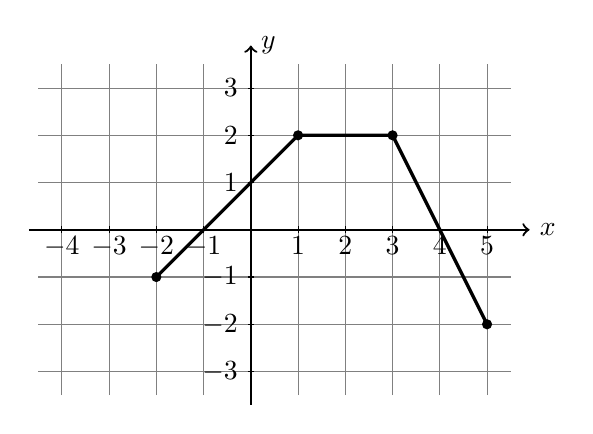
\begin{tikzpicture}[scale=0.6]

\draw [thin, color=gray, xstep=1.0cm, ystep=1.0cm] (-4.5,-3.5) grid (5.5,3.5);

\foreach \x in {-4,-3,-2,-1,1,2,3,4,5}
\draw[shift={(\x,0)}, color=black] (0pt,-2pt) -- (0pt,2pt) node[below] {$\x$};

\foreach \y in {-3,-2,-1,1,2,3}
\draw[shift={(0,\y)}, color=black] (2pt,0pt) -- (-2pt,0pt) node[left] {$\y$};

\draw [thick, ->] (-4.7,0) -- (5.9,0) node [right] {$x$};
\draw [thick, ->] (0,-3.7) -- (0,3.9) node [right] {$y$};

% image graph y = f(x-1)
\draw [very thick] (-2,-1) -- (1,2) -- (3,2) -- (5,-2);
\foreach \pt in {(-2,-1),(1,2),(3,2),(5,-2)}
  \node[circle, fill, inner sep=1.3pt] at \pt {};

\end{tikzpicture}
\end{center}
\end{figure}

\emph{(Solution graph for 6(c): $y=f(x-1)$.)}

\end{enumerate}
\end{document}
